\documentclass[11pt]{article}

\usepackage{booktabs}
\usepackage{dcolumn} 
\usepackage{epstopdf}
\usepackage{fourier}
\usepackage{fullpage}
\usepackage{graphicx}
\usepackage{hyperref}
\usepackage{longtable} 
\usepackage{natbib}
\usepackage{rotating}
\usepackage{tabularx}
\usepackage{amsmath}
% \usepackage{algorithmic} 
% \usepackage{algorithm2e}

\hypersetup{
  colorlinks = TRUE,
  citecolor=blue,
  linkcolor=red,
  urlcolor=black
}

\begin{document} 

\title{Perceived Wages versus Actual Wages:\\ Some Facts from a Surveyed Convenience Sample}

\date{\today}

\author{ John J. Horton \\ Leonard N. Stern School of Business\footnote{Author contact information, datasets and code are currently or will be available at \href{http://www.john-joseph-horton.com/}{http://www.john-joseph-horton.com/}. } }
\maketitle

\begin{abstract}
\noindent  Using a convenience sample of workers, I test their perceptions of hourly wages and actual hourly wages for the top one hundred BLS occupations, as measured by employment. 
Estmation errors are decreasing in the prevelance of an occupation. 
Knowing someone who has that occupation also decreases error rates. 
There appears to be a U-shaped pattern in knowledge about occupations
Workers do not appear to know random subsets of people with an occupation: knowledge is substantially clustered. \newline 
\newline 
\noindent JEL J01, J24, J3
\end{abstract} 

\section{Introduction}

Workers need know what various occupations pay--and will pay in the future---to plan their careers. 
Misinformation could lead to poorly considered human capital investments and job search srategies. 
However, to the extent that misinformation exists, it might be readily fixed: 
several studies have highlighted the powerful effects obtainable from purely informational interventions (e.g., \cite{jensen2010perceived}, \cite{dupas2009teenagers}, \cite{card2010inequality}). 
The connection between labor market information and allocative efficiency was in part the motivation for the Knowledge of the World of Work (KWW) test, which was briefly included in the NLSY \cite{kohen1975}.  
However, the structure of the test made it more like an IQ test and revealed more about the test-taker than population level knowledge about jobs. 

Government statistical agencies do collect and disseminate wage, educational requirements and forecasts for occupations. 
However, it is unclear whether this dissemination is effective. 
The purpose of this study is to assess the accuracy of information about occupations and expore what factors mediate this accuracy. 
A convenience sample of US-based workers on their knowledge about the one hundred largest (by May 2013 OES report) occupations.  
For each occupation, participants were asked whether (1) they knew what the occupation consisted of; (2) whether they knew anyone who held that occupation; (3) their estimate of the hourly wage for that occupation and (3) whether in the future, wages and employment for that occupation would rise or fall. 

An important question is whether this convenience sample can provide insights that generalize. 
There are several things that suggest they would. 
First, \cite{TK} shows that the demographics of MTurk workers is similar to the US population at large. 
Second, we report three Google Consumer Survey results for particular occupations and find good agreement with the MTurk results. 
Google Consumer Surveys provides a nationally representative sample.   

The advantage of using MTurk is that we can cheaply build a much larger sample than would be otherwise possible. 
Our main interest is in trends and patterns rather than ``levels.'' 
 
For each occupation, 30 evaluations were performed. 
The short time taken to answer questions suggests that workers are not doing research. 
There was no incentive for correct answers. 

The focus on the analysis was to:
-characterize performance and see whether the ``wisdom of crowds'' hypotheses holds regarding occupations 
-find poorly labeled occupations in the BLS/OES 
-see what occupations are misperceived. 
-see how total employment and social knowledge mediate performance in estimating hourly wages 
-test whether social knowledge is ``segmented'' by wage  

There is substantial variation across occupations in whether they are known by the sample. 
First, individual error rates (MSE between predicted and actual hourly wage) are decreasing the total employment in that occupation. 
This is both re-assuring and unsurprising. 
Suggesting a mechanism, the more people workers know with that occupation, the better their estimates.  
Knowledge of an occupation seems to be substantially wage-biased, in that workers are more accurate when predicting the hourly wage of low-wage jobs. 
This is true in percentages.  
The wisdom of crowds hypotheses suggests that combining the noisy signals of a large number of individuals can lead to very accurate predictions. 
This is more or less the case here: the mean worker rating for each occupation explains 70\% of the variation in actual log hourly wages.  

%% This was the justification for including the Knowledge of the World of Work (KWW) test in the NLSY. 
%% The original KWW consisted of matching job descriptions to job titles and a section of relative comparisons of wages. 
%% The KWW was predictive of positive future economic success and was correlated with higher wages, greater tenure etc \citep{kohen1975133}. 
%% It is unclear whether KWW was just measuring intelligence of ability---KWW is sometimes used as an instrument for IQ to deal with measurement error. 

%\cite{snowberg2011prediction}
% 

\section{Results}

The sample of workers answering questions on MTurk. 
What we lack in representativeness, we gain in numbers. 

If a pattern or causal effect exists in one population, there is always a question of generalizability. 

\subsection{Discussion} 
What if the sample of respondents is just a sample of low-wage workers? 

- We can ask workers for their incomes 
- We can show in the literature that this is not a particularly biased group 
- We can use Google Survey, a nationally representative sample, to adjust 

What if high-way jobs are just less common?
Controlling for the total employment in that category does not make the effect go away. 

What if the hourly/annual salary throws things off? 

Do high-way jobs just have more variance? 

\subsection{Knowledge of what different occupations are} 

In Figure~\ref{fig:knoweldge_by_occupation}, we plot the mean knowledge index by occupations.  

\begin{figure}
\caption{Self-reported knowledge by BLS occupation title \label{fig:knowledge_by_occupation}} 
\centering
\begin{minipage}{0.95 \linewidth}
\includegraphics[width = \linewidth]{./plots/knowledge_by_occupation.pdf}
\end{minipage}  
\end{figure} 

In Figure~\ref{fig:knowledge_by_wage} we show the fraction of respondents reporting that they know what an occupation is, binned by hourly wage. 
A clear U-shaped pattern is apparent: respondnents know more about low- and high-wage occupations, but less about the middle. 
This probably reflects universal experience with low-wage jobs like waitressing and cleaning and high-wage professional jobs like doctor and lawyer. 

\begin{figure}
\caption{Hourly wage and occupational knowledge \label{fig:knowledge_by_wage}} 
\centering
\begin{minipage}{0.95 \linewidth}
\includegraphics[width = \linewidth]{./plots/knowledge_by_wage.pdf}
\end{minipage}  
\end{figure} 

\begin{figure}
\caption{Mean errors by occupation \label{fig:errors}} 
\centering
\begin{minipage}{0.95 \linewidth}
\includegraphics[width = \linewidth]{./plots/error_type.pdf}
\end{minipage}  
\end{figure} 

\subsection{Personal knowledge of someone working with an occupation} 

\begin{figure}
\caption{Social index by BLS occupation title} \label{fig:social_by_occupation}  
\centering
\begin{minipage}{0.95 \linewidth}
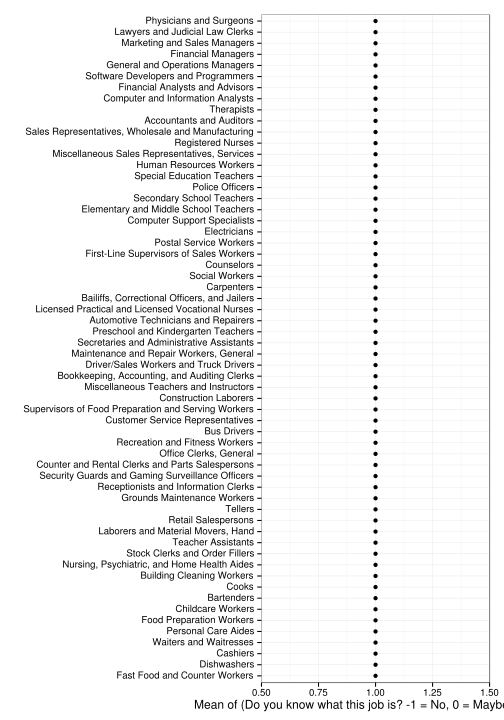
\includegraphics[width = \linewidth]{./plots/social_by_occupation.pdf}
\end{minipage}  
\end{figure} 

\subsection{Prediction} 

In Table~\ref{tab:error_prediction} we regress a measure of error in hourly wage estimates on a number of predictors. 
Column (1) reports an OLS regression, while in Columns (2) and (3) are multilevel models: 
Column (2) includes an occupations-specific random effect, while Column (3) includes both an occupation- and worker-specific random effect. 

From Column (1), we can see that knowing what the occupation consists of is negatively correlated with the error rate, as knowing more people who have that occupation. 
Error is decreasing in the total empoyment in that occupation, though presumably both knowledge measures are mediating this total employment effect. 
In Column (2), when we control for occupation, we cannot include the total employment measure. 

With occupation-specific controls, knowing what the occupation is still reduces error, but the effect is cut in 1/3. 
Much of the variation in error rates is seemingly explained by occupation-specific variation in what a job consists of. 
With these occupation-specific controls, social knowledge becomes slightly more effective at reducing error rates. 
In Column (3), the inclusion of an individual specific random effect does not lower the effect of social knowledge. 
This rules out the possibility that workers that know lots of people are somehow just better at predicting wage rates generically.  

\begin{table}
\centering 
\caption{Worker error (absolute value of difference in log wages) \label{tab:error_prediction}}
%%%%%%%%%%%%%%%%%%%%%%%%%%%%%%%%%%%%%%%%%%%%%%%%%%%%%%%%%%%%%%%%%%%%%%%%%%%%%%%%%%%%%%%%%%%%%%
%
% Calls:
% (1):  lm(formula = error ~ social + know + log(tot.emp), data = mturk.df) 
% (2):  lmer(formula = error ~ social + know + (1 | title), data = mturk.df) 
% (3):  lmer(formula = error ~ social + know + (1 | title) + (1 | WorkerId), data = mturk.df) 
%
%%%%%%%%%%%%%%%%%%%%%%%%%%%%%%%%%%%%%%%%%%%%%%%%%%%%%%%%%%%%%%%%%%%%%%%%%%%%%%%%%%%%%%%%%%%%%%
\begin{tabular}{lcD{.}{.}{7}cD{.}{.}{7}cD{.}{.}{7}}
\toprule
&&\multicolumn{1}{c}{(1)} && \multicolumn{1}{c}{(2)} && \multicolumn{1}{c}{(3)}\\
\midrule
(Intercept)                &  &  0.627^{***} &&  0.363^{***} &&  0.369^{***}\\
                           &  &  (0.110)     &&  (0.019)     &&  (0.020)    \\
Knows someone with the job &  &  -0.008      && -0.011^{*}   && -0.010^{*}  \\
                           &  &  (0.005)     &&  (0.005)     &&  (0.005)    \\
Knows what job consists of &  & -0.035^{***} &&  -0.010      &&  -0.009     \\
                           &  &  (0.010)     &&  (0.009)     &&  (0.010)    \\
Log total employment       &  & -0.018^{*}   &&              &&             \\
                           &  &  (0.008)     &&              &&             \\
Var((Intercept)|title)     &  &              &&   0.024      &&   0.024     \\
                           &  &              &&              &&             \\
Var(|Residual)             &  &              &&   0.061      &&   0.058     \\
                           &  &              &&              &&             \\
Var((Intercept)|WorkerId)  &  &              &&              &&   0.004     \\
                           &  &              &&              &&             \\
\midrule
R-squared                  &  &      0.011   &&              &&             \\
adj. R-squared             &  &      0.010   &&              &&             \\
sigma                      &  &      0.290   &&              &&             \\
F                          &  &     10.679   &&              &&             \\
p                          &  &      0.000   &&              &&             \\
Log-likelihood             &  &   -535.826   &&   -201.886   &&   -163.483  \\
Deviance                   &  &    248.486   &&    403.771   &&    326.965  \\
AIC                        &  &   1081.652   &&    413.771   &&    338.965  \\
BIC                        &  &   1111.603   &&    443.723   &&    374.907  \\
N                          &  &   2952       &&   2952       &&   2952      \\
\bottomrule
\end{tabular}
  
\end{table} 

Figure~\ref{fig:by_occupation_boxplots} shows the mean and median wage for each occupation, along with a boxplot (without outliers) the wage predictions. 
The x-axis is on a log scale. 
We can see that individuals systematically underestimate the returns at high end of the labor market. 
This can be seen even more clearly in Figure~\ref{fig:prediction_scatter}, in which we plot mean predicted wages verus actual hourly wages. 

The data points are also labeled with prediction outliers. 
It is interesting to note that a common feature of occupations where respondents underestimate are managerial occupations.  
The only substantial overestimate is the wages for home health aides. 
This could represent a mistaken association of ``health'' with high-skilled (and hence high-paying). 

\begin{figure}
\caption{Box plots showing distribution of respondent hourly wage perceptions by occupation \label{fig:by_occupation_boxplots}} 
\centering 
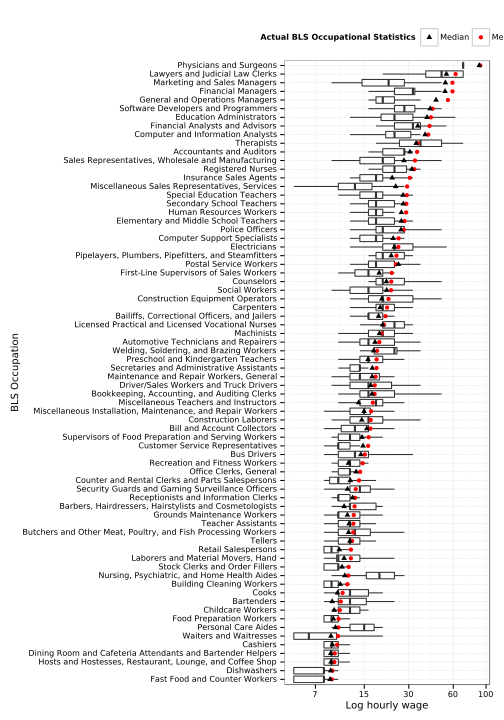
\includegraphics[width = \linewidth]{./plots/box_plots_by_occupation.pdf} 
\end{figure} 

\begin{figure}
\caption{Perceived hourly wages versus actual hourly wages \label{fig:prediction_scatter}} 
\centering 
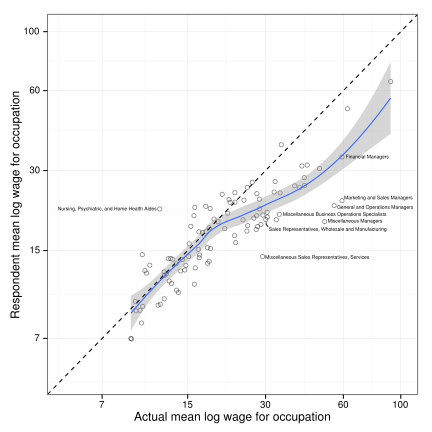
\includegraphics[width = \linewidth]{./plots/predicted_v_actual.pdf} 
\end{figure} 

We saw from Table~TK that nowing someone who works in an occupation reduces uncertainty about that occupation. 
A natural question is whether workers are stratified in their knowledge. 
In other words, for each occupation, does a worker's probability of knowing someone in that occupation depend upon the wages of other occupations for which they said they knew someone? 

In Table~\ref{tab:clustering}, we explore whether respondents differ in their knowledge of someone working in a job based on the wages of people they know working in other jobs. 
For each observation $i$, we compute $\bar{w}_{-i}$, which is the mean wage of other occupations that worker evaluated in which they said they did know someone.  
We then regress: 
\begin{equation}
\mbox{know}_i = \beta_0 + \beta_1 \log w_i + \beta_2 \log \bar{w}_{-i} + \beta_3 \log w_i \times \log \bar{w}_{-i} 
\end{equation} 

Although high wages are associated with a lower probability of knowing what a job consists of, the interaction is positive. 
This suggests that respondents that reported knowing people in higher-wage occupation where more likely to know someone in the $i$th occupation if the $i$th occupation was itself higher-wage. 

\begin{table}
\centering 
\caption{Stratification in knowledge of someone working in an occupation \label{tab:clustering}}
%%%%%%%%%%%%%%%%%%%%%%%%%%%%%%%%%%%%%%%%%%%%%%%%%%%%%%%%%%%%%%%%%%%%%%%%%%%%%%%%%%%%%%%%%%%%%%%%%%%%%%%%%%%%%%%%%%%%%%%%%%%%%%%%%%%%%%%%%%%%%%
%
% Calls:
% (1):  lm(formula = I(social > -2) ~ log(actual.mean.wage) * mean.wage.others.social + log(tot.emp), data = by.worker.df) 
% (2):  lmer(formula = I(social > -2) ~ log(actual.mean.wage) * mean.wage.others.social + log(tot.emp) + (1 | WorkerId), data = by.worker.df) 
% (3):  lmer(formula = I(social > -2) ~ log(actual.mean.wage) * mean.wage.others.social + (1 | WorkerId) + (1 | title), data = by.worker.df) 
%
%%%%%%%%%%%%%%%%%%%%%%%%%%%%%%%%%%%%%%%%%%%%%%%%%%%%%%%%%%%%%%%%%%%%%%%%%%%%%%%%%%%%%%%%%%%%%%%%%%%%%%%%%%%%%%%%%%%%%%%%%%%%%%%%%%%%%%%%%%%%%%
\begin{tabular}{lcD{.}{.}{7}cD{.}{.}{7}cD{.}{.}{7}}
\toprule
&&\multicolumn{1}{c}{(1)} && \multicolumn{1}{c}{(2)} && \multicolumn{1}{c}{(3)}\\
\midrule
(Intercept)                                             &  &  3.574^{***} &&  2.699^{**}  &&  4.880^{***}\\
                                                        &  &  (1.015)     &&  (0.977)     &&  (0.929)    \\
log(actual.mean.wage)                                   &  & -1.510^{***} && -1.244^{***} && -1.390^{***}\\
                                                        &  &  (0.327)     &&  (0.306)     &&  (0.296)    \\
mean.wage.others.social                                 &  & -1.626^{***} && -1.318^{***} && -1.406^{***}\\
                                                        &  &  (0.332)     &&  (0.320)     &&  (0.307)    \\
log(tot.emp)                                            &  &  0.131^{***} &&  0.131^{***} &&             \\
                                                        &  &  (0.015)     &&  (0.014)     &&             \\
log(actual.mean.wage) $\times$ mean.wage.others.social &  &  0.504^{***} &&  0.415^{***} &&  0.447^{***}\\
                                                        &  &  (0.109)     &&  (0.102)     &&  (0.098)    \\
Var((Intercept)|WorkerId)                               &  &              &&   0.045      &&   0.040     \\
                                                        &  &              &&              &&             \\
Var(|Residual)                                          &  &              &&   0.198      &&   0.179     \\
                                                        &  &              &&              &&             \\
Var((Intercept)|title)                                  &  &              &&              &&   0.027     \\
                                                        &  &              &&              &&             \\
\midrule
R-squared                                               &  &      0.040   &&              &&             \\
adj. R-squared                                          &  &      0.039   &&              &&             \\
sigma                                                   &  &      0.489   &&              &&             \\
F                                                       &  &     26.252   &&              &&             \\
p                                                       &  &      0.000   &&              &&             \\
Log-likelihood                                          &  &  -1754.623   &&  -1609.371   &&  -1555.602  \\
Deviance                                                &  &    596.067   &&   3218.743   &&   3111.204  \\
AIC                                                     &  &   3521.245   &&   3232.743   &&   3125.204  \\
BIC                                                     &  &   3556.182   &&   3273.503   &&   3165.964  \\
N                                                       &  &   2497       &&   2497       &&   2497      \\
\bottomrule
\end{tabular}
 
\end{table} 


\begin{figure}
\caption{Wage trends} 
\centering
\begin{minipage}{0.85 \linewidth}
\includegraphics[width = \linewidth]{./plots/wage_trends.png}
\end{minipage}  
\end{figure} 


%% \begin{figure}
%% \caption{Knowledge by total employment} 
%% \centering
%% \begin{minipage}{0.85 \linewidth}
%% \includegraphics[width = \linewidth]{./plots/knowledge_emp.png}
%% \end{minipage}  
%% \end{figure} 


%% latex table generated in R 3.0.2 by xtable 1.7-1 package
% Sun Nov 10 03:27:45 2013
\begin{table}[ht]
\centering
\begin{tabular}{rll}
  \hline
 &      OES &      MTSO \\ 
  \hline
1 & Min.   :0.0000   & Min.   :18.05   \\ 
  2 & 1st Qu.:0.5000   & 1st Qu.:28.54   \\ 
  3 & Median :0.7000   & Median :32.14   \\ 
  4 & Mean   :0.7152   & Mean   :34.29   \\ 
  5 & 3rd Qu.:0.9000   & 3rd Qu.:39.77   \\ 
  6 & Max.   :1.4000   & Max.   :60.57   \\ 
   \hline
\end{tabular}
\caption{RSE for Hourly Wages in OES and MTSO datasets (all obs.)} 
\label{tab:rse_oes_mtso1}
\end{table}

%% latex table generated in R 3.0.2 by xtable 1.7-1 package
% Sun Nov 10 03:30:09 2013
\begin{table}[ht]
\centering
\begin{tabular}{rll}
  \hline
 &      OES &      MTSO \\ 
  \hline
1 & Min.   :0.0000   & Min.   :15.01   \\ 
  2 & 1st Qu.:0.5000   & 1st Qu.:25.82   \\ 
  3 & Median :0.7000   & Median :30.96   \\ 
  4 & Mean   :0.7173   & Mean   :32.69   \\ 
  5 & 3rd Qu.:0.9000   & 3rd Qu.:40.00   \\ 
  6 & Max.   :1.4000   & Max.   :65.93   \\ 
  7 &  & NA's   :2   \\ 
   \hline
\end{tabular}
\caption{RSE for Hourly Wages in OES and MTSO datasets (filtered)} 
\label{tab:rse_oes_mtso2}
\end{table}


%% \begin{small} 
%% %%%%%%%%%%%%%%%%%%%%%%%%%%%%%%%%%%%%%%%%%%%%%%%%%%%%%%%%%%%%%%%%%%%%%%%%%%%%%%%%%%%%%%%%%%%%%%%%%%%%%%%%%%%%%%%%%%%%%%%%%%%%%
%
% Calls:
% 1:  glm(formula = error ~ know * social + log(TOT_EMP) + log(H_WAGE), data = mturk.df) 
% 2:  glm(formula = error ~ know * social + log(H_WAGE), data = mturk.df) 
% 3:  glm(formula = error ~ social + log(H_WAGE) + log(TOT_EMP), data = mturk.df) 
% 4:  lmer(formula = error ~ know * social + log(TOT_EMP) + log(H_WAGE) + (1 | Input.Title), data = mturk.df) 
% 5:  glm(formula = error ~ know * social + log(TOT_EMP) + log(H_WAGE) + I(log(Answer.wage) > 3), data = mturk.df) 
%
%%%%%%%%%%%%%%%%%%%%%%%%%%%%%%%%%%%%%%%%%%%%%%%%%%%%%%%%%%%%%%%%%%%%%%%%%%%%%%%%%%%%%%%%%%%%%%%%%%%%%%%%%%%%%%%%%%%%%%%%%%%%%
\begin{tabular}{lcD{.}{.}{7}cD{.}{.}{7}cD{.}{.}{7}cD{.}{.}{7}cD{.}{.}{7}}
\toprule
&&\multicolumn{1}{c}{1} && \multicolumn{1}{c}{2} && \multicolumn{1}{c}{3} && \multicolumn{1}{c}{4} && \multicolumn{1}{c}{5}\\
\midrule
(Intercept)                  &  & -0.635^{***} && -0.291^{***} && -0.594^{***} && -0.617^{*}   && -0.783^{***}\\
                             &  &  (0.122)     &&  (0.044)     &&  (0.119)     &&  (0.291)     &&  (0.118)    \\
know                         &  &   0.041      &&   0.045      &&              &&   0.029      &&   0.039     \\
                             &  &  (0.032)     &&  (0.032)     &&              &&  (0.030)     &&  (0.030)    \\
social                       &  & -0.039^{*}   && -0.038^{*}   && -0.012^{**}  && -0.030^{*}   && -0.031^{*}  \\
                             &  &  (0.016)     &&  (0.016)     &&  (0.005)     &&  (0.015)     &&  (0.015)    \\
log(TOT_EMP)                 &  &  0.024^{**}  &&              &&  0.023^{**}  &&   0.023      &&  0.020^{**} \\
                             &  &  (0.008)     &&              &&  (0.008)     &&  (0.019)     &&  (0.008)    \\
log(H_WAGE)                  &  &  0.209^{***} &&  0.200^{***} &&  0.211^{***} &&  0.209^{***} &&  0.293^{***}\\
                             &  &  (0.010)     &&  (0.010)     &&  (0.010)     &&  (0.026)     &&  (0.011)    \\
know $\times$ social        &  &   0.031      &&  0.032^{*}   &&              &&   0.020      &&   0.027     \\
                             &  &  (0.016)     &&  (0.016)     &&              &&  (0.015)     &&  (0.016)    \\
Var((Intercept)|Input.Title) &  &              &&              &&              &&   0.013      &&             \\
                             &  &              &&              &&              &&              &&             \\
Var(|Residual)               &  &              &&              &&              &&   0.061      &&             \\
                             &  &              &&              &&              &&              &&             \\
I(log(Answer.wage) > 3)      &  &              &&              &&              &&              && -0.206^{***}\\
                             &  &              &&              &&              &&              &&  (0.013)    \\
\midrule
Aldrich-Nelson R-sq.         &  &      0.011   &&      0.011   &&      0.011   &&              &&      0.017  \\
McFadden R-sq.               &  &      0.132   &&      0.129   &&      0.129   &&              &&      0.203  \\
Cox-Snell R-sq.              &  &      0.011   &&      0.011   &&      0.011   &&              &&      0.017  \\
Nagelkerke R-sq.             &  &      0.136   &&      0.134   &&      0.134   &&              &&      0.210  \\
phi                          &  &      0.074   &&      0.074   &&      0.074   &&              &&      0.068  \\
Likelihood-ratio             &  &     33.039   &&     32.365   &&     32.566   &&              &&     51.068  \\
p                            &  &      0.000   &&      0.000   &&      0.000   &&              &&      0.000  \\
Log-likelihood               &  &   -343.627   &&   -348.183   &&   -348.287   &&   -183.829   &&   -216.304  \\
Deviance                     &  &    218.147   &&    218.822   &&    219.290   &&    367.658   &&    200.118  \\
AIC                          &  &    701.254   &&    708.367   &&    706.574   &&    383.658   &&    448.608  \\
BIC                          &  &    743.186   &&    744.308   &&    736.538   &&    431.580   &&    496.530  \\
N                            &  &   2952       &&   2952       &&   2960       &&   2952       &&   2952      \\
\bottomrule
\end{tabular}
 
%% \end{small} 

%% \begin{tiny} 
%% \caption{Know anyone}
%% %%%%%%%%%%%%%%%%%%%%%%%%%%%%%%%%%%%%%%%%%%%%%%%%%%%%%%%%%%%%%%%%%%%%%%%%%%%%%%%%%%%%%%%%%%%%%%%%%%%%%%%%%%%%%%%%%%%%%
%
% Calls:
% 1:  glm(formula = I(Answer.know_anyone != "0") ~ log(TOT_EMP), family = "binomial", data = mturk.df) 
% 2:  glm(formula = I(Answer.know_anyone != "0") ~ log(H_WAGE), family = "binomial", data = mturk.df) 
% 3:  glm(formula = I(Answer.know_anyone != "0") ~ log(H_WAGE) + log(TOT_EMP), family = "binomial", data = mturk.df) 
% 4:  glm(formula = I(Answer.know_anyone != "0") ~ log(H_WAGE) * log(TOT_EMP), family = "binomial", data = mturk.df) 
%
%%%%%%%%%%%%%%%%%%%%%%%%%%%%%%%%%%%%%%%%%%%%%%%%%%%%%%%%%%%%%%%%%%%%%%%%%%%%%%%%%%%%%%%%%%%%%%%%%%%%%%%%%%%%%%%%%%%%%
\begin{tabular}{lcD{.}{.}{7}cD{.}{.}{7}cD{.}{.}{7}cD{.}{.}{7}}
\toprule
&&\multicolumn{1}{c}{1} && \multicolumn{1}{c}{2} && \multicolumn{1}{c}{3} && \multicolumn{1}{c}{4}\\
\midrule
(Intercept)                        &  & -6.916^{***} &&    0.423     && -6.988^{***} &&    1.333    \\
                                   &  &  (0.755)     &&   (0.223)    &&  (0.879)     &&   (4.593)   \\
log(TOT_EMP)                       &  &  0.502^{***} &&              &&  0.505^{***} &&   -0.110    \\
                                   &  &  (0.056)     &&              &&  (0.058)     &&   (0.338)   \\
log(H_WAGE)                        &  &              &&  -0.177^{*}  &&   0.012      &&   -2.913    \\
                                   &  &              &&   (0.073)    &&  (0.077)     &&   (1.590)   \\
log(H_WAGE) $\times$ log(TOT_EMP) &  &              &&              &&              &&    0.217    \\
                                   &  &              &&              &&              &&   (0.118)   \\
\midrule
Aldrich-Nelson R-sq.               &  &      0.028   &&      0.002   &&      0.028   &&      0.029  \\
McFadden R-sq.                     &  &      0.020   &&      0.001   &&      0.020   &&      0.021  \\
Cox-Snell R-sq.                    &  &      0.028   &&      0.002   &&      0.028   &&      0.029  \\
Nagelkerke R-sq.                   &  &      0.037   &&      0.003   &&      0.037   &&      0.039  \\
phi                                &  &      1.000   &&      1.000   &&      1.000   &&      1.000  \\
Likelihood-ratio                   &  &     84.108   &&      5.950   &&     84.133   &&     87.543  \\
p                                  &  &      0.000   &&      0.015   &&      0.000   &&      0.000  \\
Log-likelihood                     &  &  -2011.313   &&  -2050.392   &&  -2011.300   &&  -2009.595  \\
Deviance                           &  &   4022.626   &&   4100.784   &&   4022.601   &&   4019.191  \\
AIC                                &  &   4026.626   &&   4104.784   &&   4028.601   &&   4027.191  \\
BIC                                &  &   4038.618   &&   4116.776   &&   4046.589   &&   4051.175  \\
N                                  &  &   2969       &&   2969       &&   2969       &&   2969      \\
\bottomrule
\end{tabular}
 
%% \end{tiny} 

\bibliographystyle{aer}
\bibliography{kwow.bib}

\end{document} 
